\documentclass[12pt,letterpaper]{article}
\usepackage{fontspec}
\usepackage[spanish,es-noshorthands,es-tabla,es-lcroman]{babel}
\usepackage{../plantilla/latex/unab_reporte}
% Generado por compilar.py desde datos/datos.md. No editar.
\newcommand{\TituloTrabajo}{CircuitRush: Restaura la Energía}
\newcommand{\SubtituloTrabajo}{Vibecoding Guiado: Desarrollo de una Aplicación o Mini-Juego con IA como Copiloto}
\newcommand{\TituloCorto}{CircuitRush · KODIGO}
\newcommand{\Institucion}{KODIGO Academy}
\newcommand{\Facultad}{AI for Developers}
\newcommand{\Asignatura}{AI for Developers Jr. 3 — KODIGO Academy}
\newcommand{\Docente}{No indicado en la consigna}
\newcommand{\Grupo}{Actividad individual}
\newcommand{\LugarFecha}{Actividad de Semana 2}
\newcommand{\NombreFirma}{Jaime Berrios}
\newcommand{\Integrantes}{%
Jaime Fernando Berrios Ortiz & No aplica \\
}

\makeatletter
\newcommand{\cita}[2][]{(\csname autorp@#2\endcsname, \csname anio@#2\endcsname\if\relax\detokenize{#1}\relax\else, #1\fi)}
\newcommand{\citatexto}[2][]{\csname autorn@#2\endcsname\ (\csname anio@#2\endcsname\if\relax\detokenize{#1}\relax\else, #1\fi)}
\newcommand{\citas}[1]{(%
  \def\citassep{}%
  \@for\@tmp:=#1\do{%
    \citassep\csname autorp@\@tmp\endcsname,~\csname anio@\@tmp\endcsname%
    \def\citassep{;~}%
  }%
)}
\makeatother
% El nombre completo procede del primer integrante; Firma conserva el nombre corto.
\def\ExtraerNombreAutor#1&#2\FinAutor{#1}
\renewcommand{\NombreAutor}{\expandafter\ExtraerNombreAutor\Integrantes\FinAutor}
\hypersetup{pdftitle={\TituloTrabajo},pdfauthor={\NombreAutor}}
\begin{document}
\portadareporte
\pagenumbering{arabic}

\section{Descripción del proyecto}
CircuitRush: Restaura la Energía es un minijuego web de lógica ambientado en una ciudad sin suministro eléctrico. El jugador debe orientar un circuito para conducir energía desde una fuente fija hasta un destino. Cada clic, o activación con Enter o Espacio, gira una pieza móvil 90 grados en sentido horario y suma un movimiento.

La propagación utiliza un recorrido en anchura (BFS): solo atraviesa casillas adyacentes cuando las conexiones coinciden en ambos extremos. Un conjunto de visitados evita recorridos repetidos y el color cian identifica las piezas energizadas. Se gana al alcanzar el destino y se pierde al agotarse el tiempo. Ambos resultados bloquean el tablero y permiten reintentar.

Existen tres niveles fijos: Encendido, de $4\times4$ y 120 segundos; Reconexión, de $5\times5$ y 180 segundos; y Sobrecarga, de $6\times6$ y 240 segundos. Completar uno desbloquea el siguiente. El reloj comienza con el primer giro válido y calcula el tiempo transcurrido real. Solo se puntúa al ganar:
\[
P=\max(0,\;1000+10s-20m),
\]
donde $s$ son los segundos restantes y $m$ los movimientos. Cada nivel conserva su mejor puntuación y menor número de movimientos en \texttt{localStorage}, junto con los desbloqueos; no se guarda la partida en curso.

Python y Flask sirven la página y sus archivos; HTML5 define la estructura, CSS3 presenta las piezas y JavaScript Vanilla controla la interacción. No hay cuentas, base de datos ni IA dentro del juego. La IA apoyó la programación y validación; Antigravity fue el entorno de programación asistida utilizado durante el desarrollo.

La actividad corresponde a la Semana 2 del curso AI for Developers Jr. 3 de KODIGO Academy. El trabajo presenta la evolución de una aplicación funcional, el uso progresivo de prompts y la validación crítica del código generado.

\clearpage
\section{Evidencia de vibecoding}
Se utilizaron tres prompts progresivos: funcionamiento, presentación y ampliación de jugabilidad. A continuación se explica qué se solicitó, por qué se refinó la instrucción y qué resultado se obtuvo. Los textos completos se incluyen en el material de respaldo al final del documento (página~\pageref{anexo:prompts}).

\textbf{Prompt 01: desarrollo del MVP funcional}\par
\textbf{Objetivo y solicitud.} Crear un tablero reproducible de $4\times4$, rotaciones horarias, conexiones recíprocas, propagación BFS o DFS, contador, victoria y reinicio, con Flask y JavaScript Vanilla. Exigió pruebas y resultados reales; excluyó temporizadores y ampliaciones prematuras.

\textbf{Motivo y resultado.} Acotar la primera versión permitió comprobar la mecánica antes de ampliarla. Se implementaron estado, conexiones, propagación y giro, además de siete pruebas iniciales. La figura~\ref{fig:mvp} muestra la interfaz funcional.

\textbf{Prompt 02: rediseño visual futurista y mejoras UX}\par
\textbf{Objetivo y solicitud.} Inspeccionar y conservar el MVP, mejorar la jerarquía visual, los estados eléctricos, las animaciones, el modal, el teclado y la adaptación responsive, sin agregar niveles ni reloj.

\textbf{Motivo y resultado.} El refinamiento abordó la claridad visual sobre una lógica ya verificable. Se incorporaron la consola energética, indicadores de conexión, brillo, transiciones y foco visible, respetando movimiento reducido. La figura~\ref{fig:rediseno} permite comparar el resultado con el MVP.

\textbf{Prompt 03: niveles, temporizador, puntuación y récords}\par
\textbf{Objetivo y solicitud.} Añadir tres tamaños de tablero, soluciones verificadas mediante giros legales, reloj basado en tiempo real, puntuación explicable, récords locales, desbloqueo y resultados de victoria o derrota. Exigió conservar las siete pruebas y comprobar datos corruptos y bloqueos.

\textbf{Motivo y resultado.} Sobre la interfaz anterior se amplió la progresión y la repetición de partidas. El código contiene tres configuraciones resolubles, una sesión que gestiona el reloj y almacenamiento tolerante a fallos. Las figuras~\ref{fig:niveles} y~\ref{fig:puntos} documentan esos cambios.

\clearpage
\section{Iteración y mejora}
El desarrollo se organizó en tres etapas para controlar el alcance y conservar el funcionamiento anterior. La tabla~\ref{tab:iteraciones} resume los cambios y las evidencias de cada una.
\begin{table}[htbp]
\centering
\caption{Evolución de CircuitRush}
\label{tab:iteraciones}
\begin{tabularx}{\linewidth}{@{}p{1.9cm}XX@{}}
\toprule
\textbf{Iteración} & \textbf{Mejora principal} & \textbf{Evidencia} \\
\midrule
01 & Tablero $4\times4$, BFS, giros, victoria y reinicio. & Siete pruebas iniciales y captura del MVP. \\
02 & Rediseño, estados eléctricos, animaciones, teclado y responsive. & Capturas Firefox y pruebas de foco y movimiento reducido. \\
03 & Niveles, reloj, puntos, récords y desbloqueo. & Diecinueve pruebas y capturas de niveles y puntuación. \\
\bottomrule
\end{tabularx}
\par\smallskip{\small Nota. Síntesis del código y del registro de iteraciones del repositorio.}
\end{table}

Las figuras~\ref{fig:mvp} y~\ref{fig:rediseno} muestran el paso de los indicadores básicos a una consola energética. Se conservaron fuente, destino y rotación.
\begin{figure}[htbp]
\begin{minipage}[t]{0.48\linewidth}
\centering
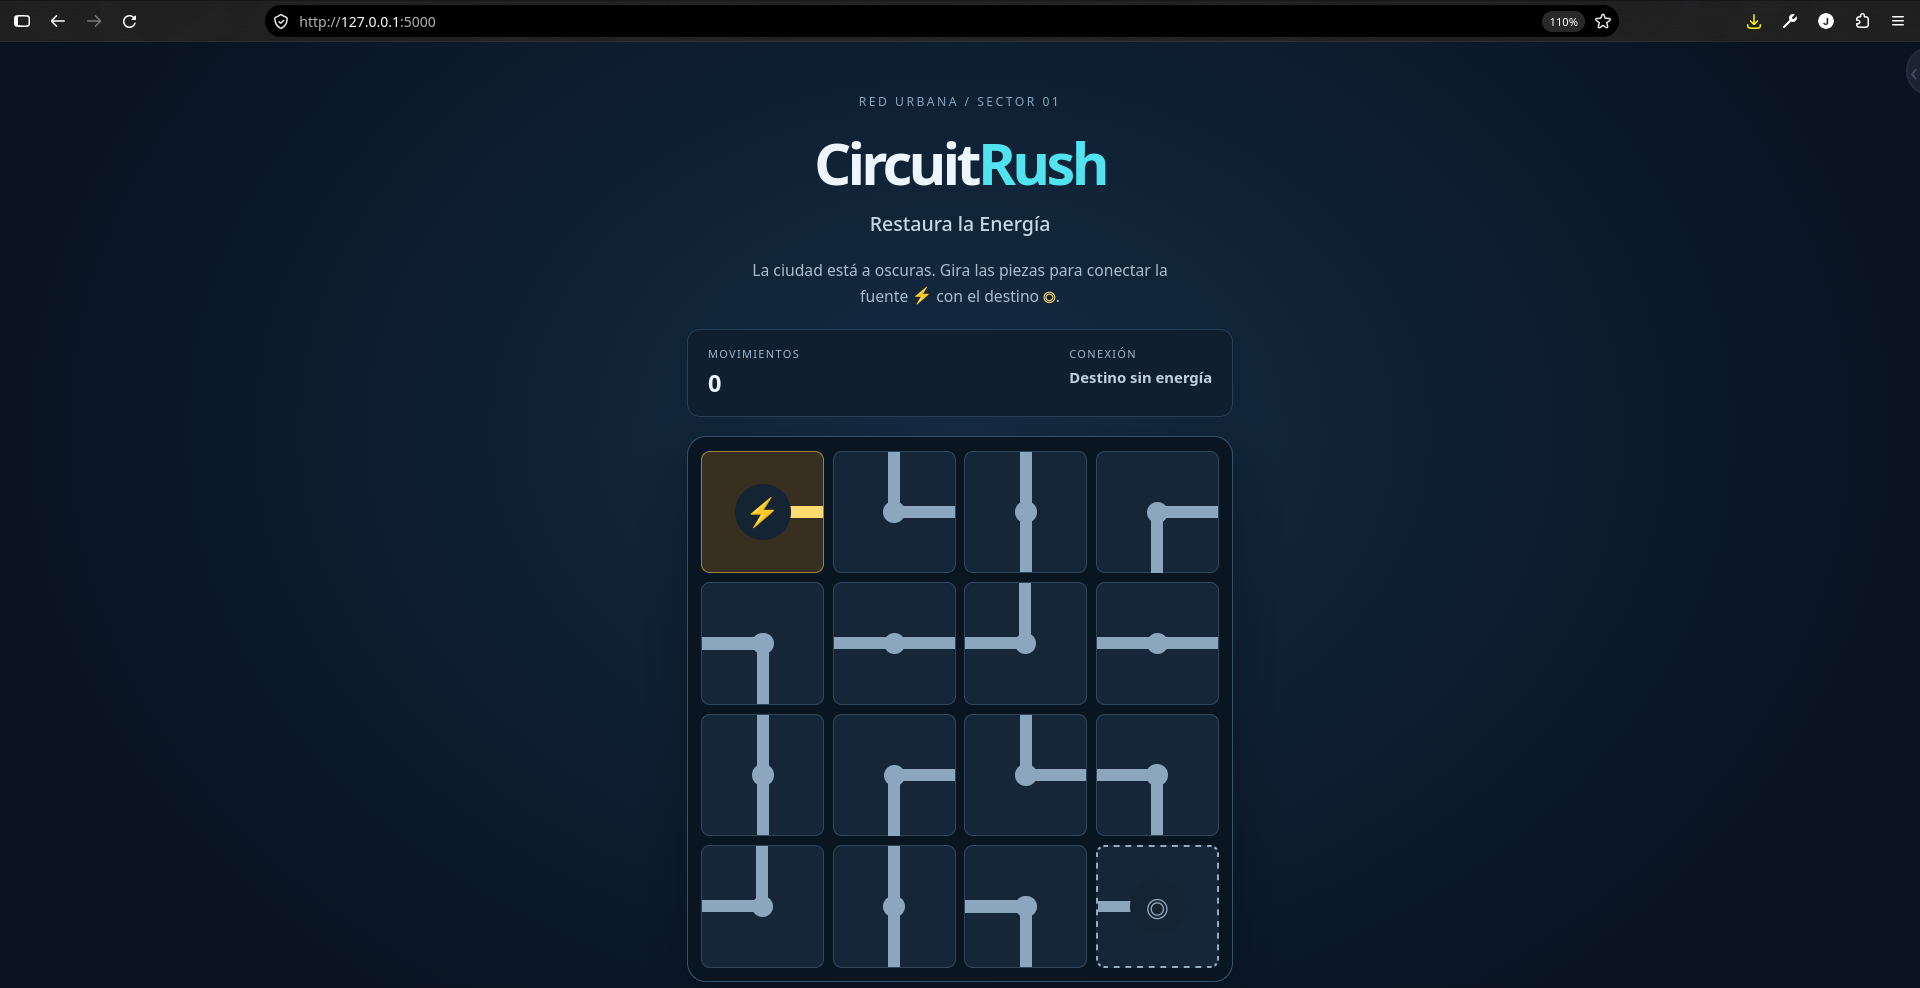
\includegraphics[width=\linewidth,height=7.1cm,keepaspectratio,trim=487bp 0bp 487bp 31bp,clip]{../assets/contenido/imagenes/Captura 01.png}
\caption{MVP: tablero inicial de 16 piezas}
\label{fig:mvp}
\end{minipage}\hfill
\begin{minipage}[t]{0.48\linewidth}
\centering
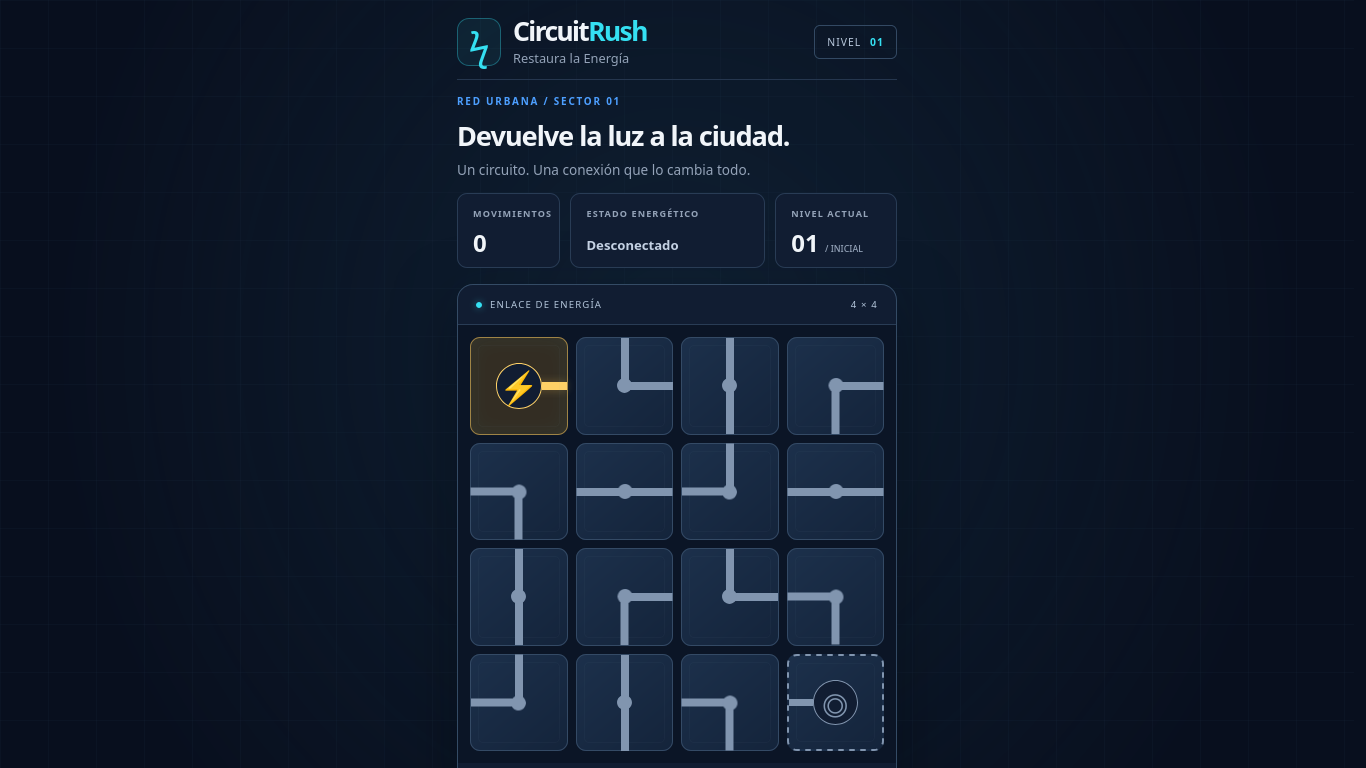
\includegraphics[width=\linewidth,height=7.1cm,keepaspectratio,trim=450bp 0bp 450bp 0bp,clip]{../assets/contenido/evidencias/iteracion-02/captura-05-interfaz-1366x768.png}
\caption{Consola rediseñada en la iteración 02}
\label{fig:rediseno}
\end{minipage}
\par\smallskip{\small Nota. Capturas propias del repositorio. Se recortan márgenes exteriores para facilitar la comparación y se conserva la proporción.}
\end{figure}

\clearpage
La tercera iteración añade selector, bloqueos y reloj. La figura~\ref{fig:niveles} muestra Reconexión; Sobrecarga amplía el tablero a $6\times6$. Las pruebas verifican que los tres niveles empiezan sin resolver y que una secuencia legal alcanza el destino. No se afirma que esas soluciones sean mínimas.
\begin{figure}[htbp]
\begin{minipage}[t]{0.48\linewidth}
\vspace{0pt}\centering
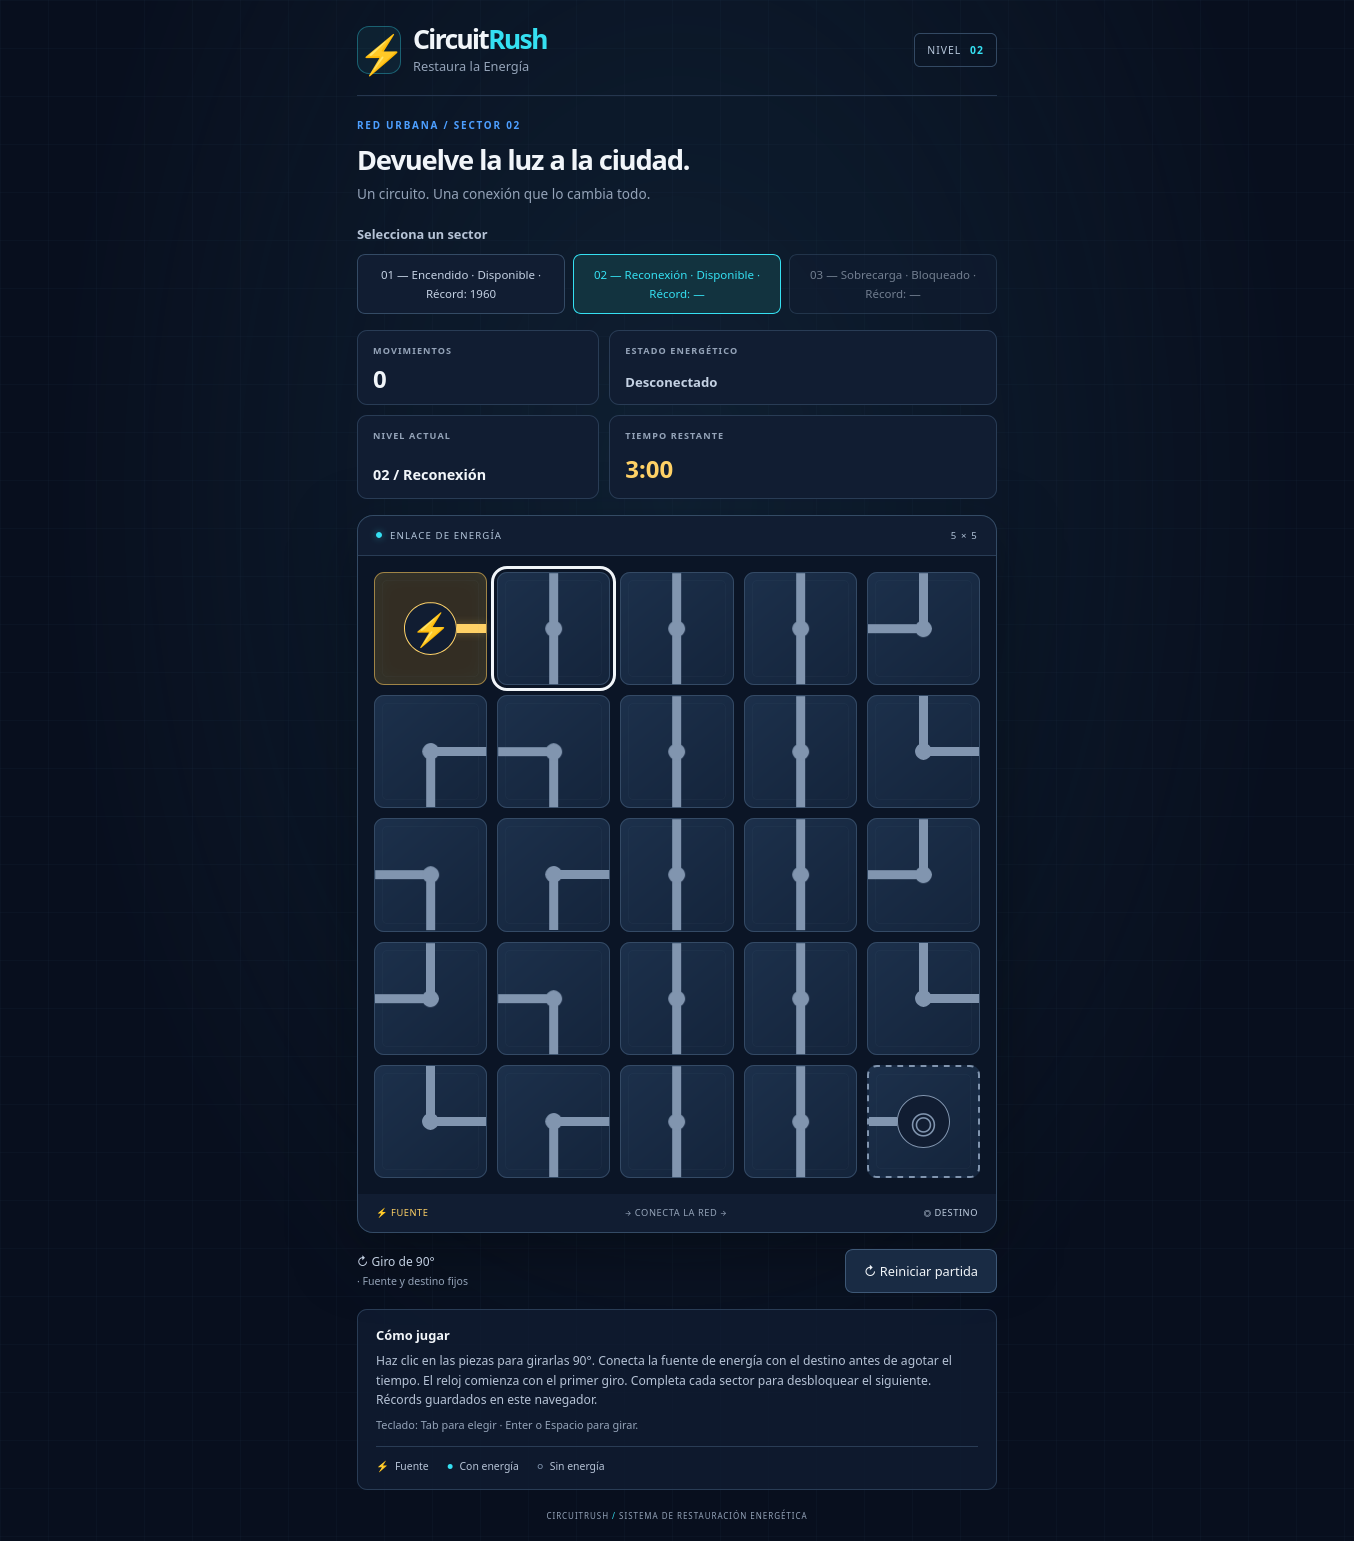
\includegraphics[width=\linewidth,height=9cm,keepaspectratio,trim=350bp 290bp 350bp 0bp,clip]{../assets/contenido/evidencias/iteracion-03/captura-10-nivel-02.png}
\caption{Reconexión: tablero $5\times5$, selector y reloj}
\label{fig:niveles}
\end{minipage}\hfill
\begin{minipage}[t]{0.48\linewidth}
\vspace{0pt}\centering
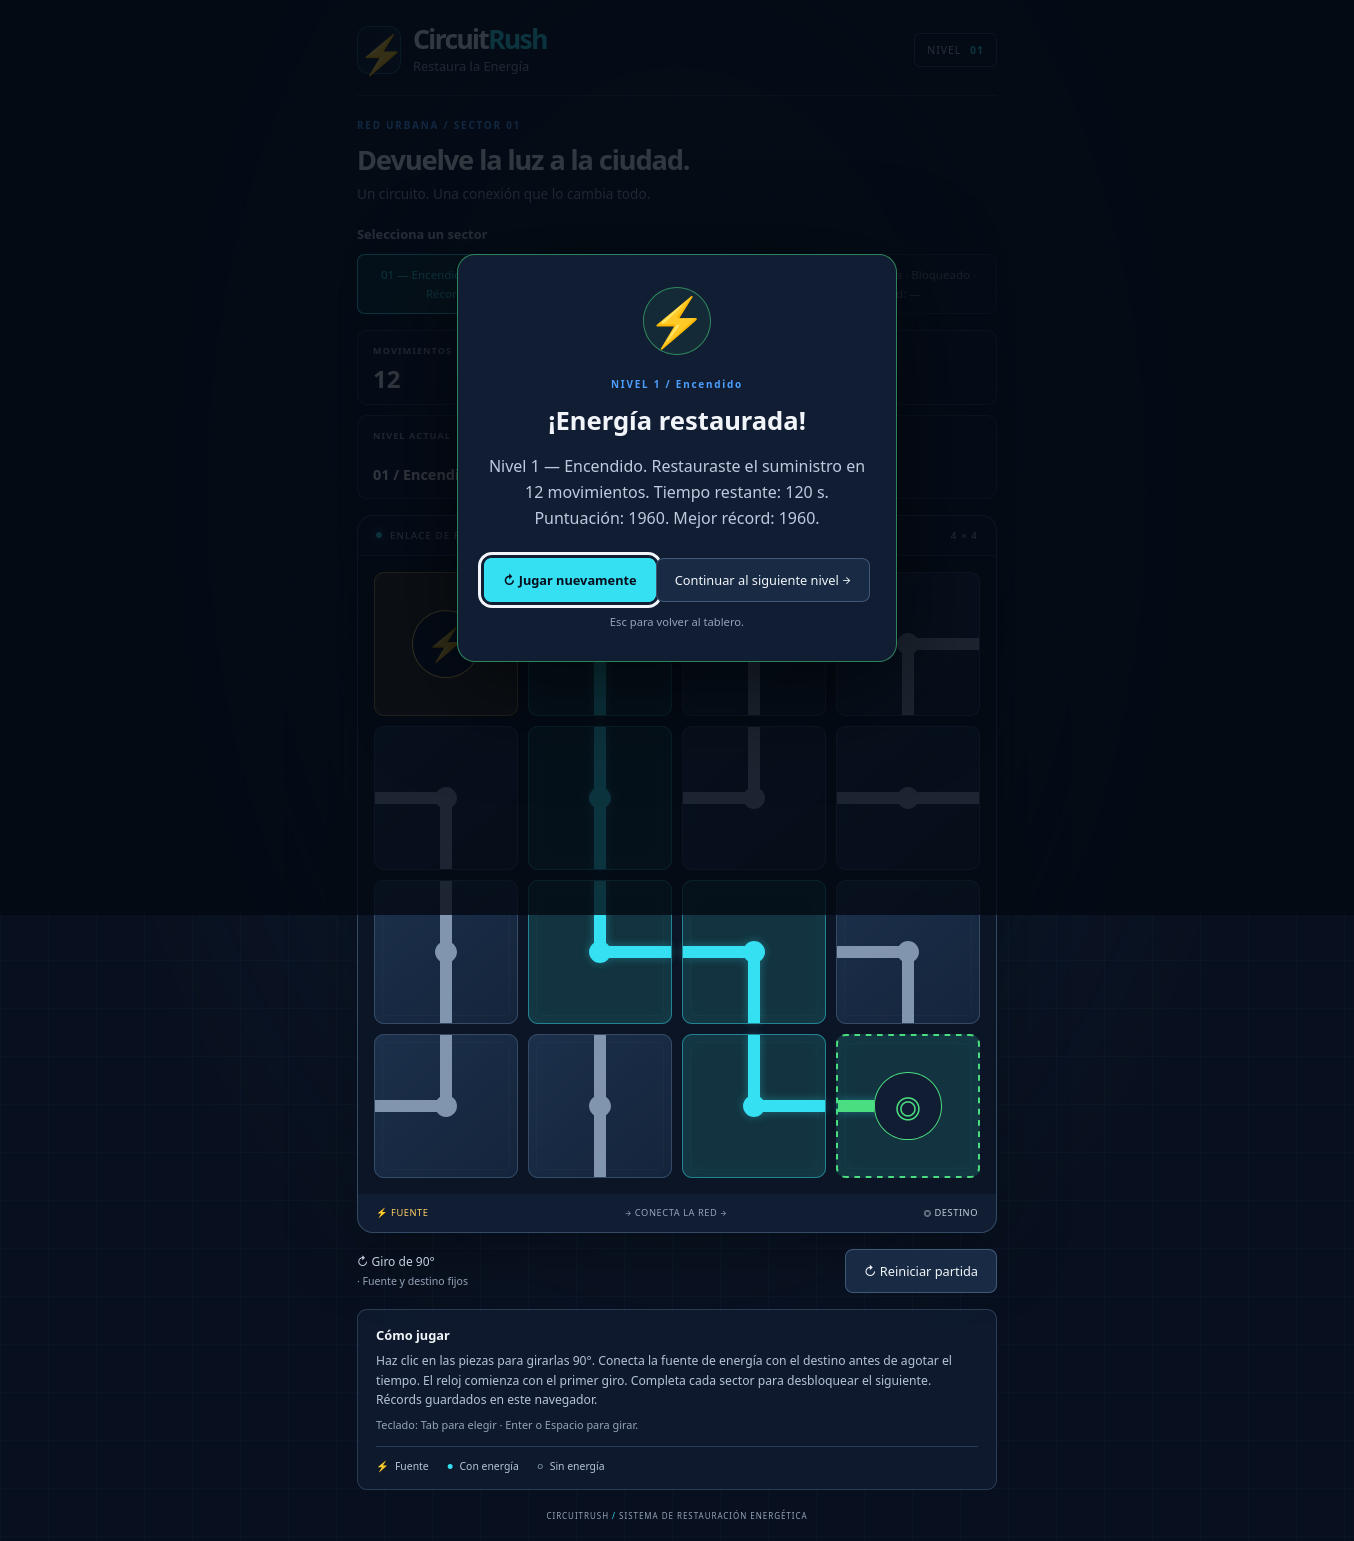
\includegraphics[width=\linewidth,height=7cm,keepaspectratio,trim=450bp 850bp 450bp 240bp,clip]{../assets/contenido/evidencias/iteracion-03/captura-13-victoria.png}
\caption{Victoria con 12 movimientos y 1960 puntos}
\label{fig:puntos}
\end{minipage}
\par\smallskip{\small Nota. Capturas 10 y 13 de Firefox, recortadas sin deformación. Se conserva el tablero completo y el modal de resultado. La puntuación mostrada es $1000+120(10)-12(20)=1960$.}
\end{figure}

\clearpage
\section{Validación del resultado}
\textbf{Resultados actuales.} Se ejecutó nuevamente el comando solicitado:
\begin{quote}\ttfamily\small node --test tests/game.test.cjs\end{quote}
Terminó correctamente y resumió \textbf{1 archivo aprobado, 0 fallidos y 0 omitidos} en este entorno. La ejecución complementaria \texttt{node tests/game.test.cjs} detalló \textbf{19 pruebas aprobadas, 0 fallidas y 0 omitidas}. Se distingue el conteo por archivo del de casos. Los registros de ejecución respaldan estos resultados.

La suite verifica giros, movimientos, conexiones recíprocas, ciclos, victoria, bloqueo y reinicio; valida los tres tamaños y sus soluciones mediante giros legales. Con reloj controlado comprueba inicio, decremento, parada, reinicio e intervalo único. También cubre puntuación no negativa, récords, recarga simulada, datos corruptos, niveles bloqueados y desbloqueo. El DOM simulado valida controles; no sustituye un navegador.

\textbf{Ejecución local.} \texttt{.venv/bin/python app.py} sirve el juego en \url{http://127.0.0.1:5000}. En esta revisión, el cliente Flask obtuvo HTTP 200 para página, CSS y JavaScript. No se presenta como una interacción visual nueva.

\textbf{Evidencia histórica y ajuste.} Las iteraciones 02 y 03 registran automatización en Firefox de teclado, victoria, continuación, recarga y movimiento reducido. En la segunda, Tab permitía abandonar el botón del modal: se añadió manejo de teclado y la repetición documentada aprobó. La tercera amplió ese manejo a la continuación. Otro ajuste fue usar una esquina en fila 4, columna 3 para permitir el recorrido; la suite actual verifica su solución de 12 movimientos.

\textbf{Alcance y límites.} Las mediciones históricas no detectaron desbordamiento a 1366, 768 y 500 píxeles. Las capturas de 390 usaron una configuración de prueba; la derrota en Firefox utilizó reloj inyectado. No se repitió esa automatización al redactar este reporte. No existen evidencias de interacción táctil física, lector de pantalla, otros navegadores o suspensión real de pestaña por el sistema operativo. Las pruebas temporales simulan retrasos. No se confunden estas comprobaciones automatizadas con pruebas manuales, ni se afirma accesibilidad total.

\clearpage
\section{Reflexión final}
\label{sec:reflexion}
\textbf{Propuesta para revisión personal.} Las respuestas siguientes requieren la revisión del autor para confirmar que describen su aprendizaje y su comprensión del código.

\textbf{a. ¿Qué aprendí utilizando IA para programar?}

Aprendí a dividir una solicitud en cambios comprobables: primero el circuito, después la interfaz y finalmente los niveles y el reloj. Pedir una función no fue suficiente; también necesité establecer cómo comprobarla, por ejemplo mediante conexiones recíprocas y una secuencia de giros que alcanzara el destino.

\textbf{b. ¿Qué ventajas y limitaciones identifiqué del vibecoding?}

La ventaja que identifico es convertir instrucciones concretas en una implementación y revisarla por etapas. La limitación es que una respuesta o captura no demuestra todo el funcionamiento. Las pruebas con un reloj simulado ayudan a revisar el vencimiento, pero no sustituyen la interacción en un móvil físico ni la revisión del código generado.

\textbf{c. ¿Qué partes del código comprendo y cuáles necesito reforzar?}

Puedo explicar la separación entre Flask, la interfaz y el estado del juego, así como la relación entre un giro y el contador. Necesito reforzar BFS, el control del tiempo y la validación del almacenamiento. Antes de presentar esta respuesta como definitiva, debo confirmar cuáles de estas partes comprendo realmente y demostrarlas con el código.

\clearpage
\section*{Material de respaldo: prompts utilizados}
\label{anexo:prompts}
Los siguientes textos reproducen íntegramente los tres prompts de desarrollo, en orden. Se conservan sus instrucciones y restricciones originales; las limitaciones de cada etapa deben interpretarse dentro de esa iteración. La tipografía compacta permite mantener separado este respaldo del reporte principal.

% Transcripción de los prompts originales. No modifica el historial.
\begingroup
\newfontfamily\FuentePrompt[Path=../assets/fuentes/]{NotoSansMono-Regular.ttf}
\FuentePrompt\fontsize{9}{12}\selectfont\singlespacing
\raggedright\setlength{\parskip}{0pt}\setlength{\parindent}{0pt}\sloppy
\phantomsection
\label{prompt:01}
{\sffamily\large\bfseries Prompt 01: texto completo\par}
\medskip
\noindent \# PROMPT 01 — CIRCUITRUSH: DESARROLLO DEL MVP FUNCIONAL\par
\par\smallskip
\noindent \#\# 1. Rol y contexto\par
\par\smallskip
\noindent Actúa como desarrollador full-stack senior, especialista en Python, Flask, HTML5, CSS3, JavaScript y desarrollo de videojuegos web 2D, con experiencia en programación asistida por inteligencia artificial y buenas prácticas de ingeniería de software.\par
\par\smallskip
\noindent Desarrollaremos **CircuitRush: Restaura la Energía**, un minijuego web de lógica y resolución de circuitos eléctricos, como parte de la actividad individual **«Vibecoding Guiado: Desarrollo de una Aplicación o Mini-Juego con IA como Copiloto»**, correspondiente al bootcamp AI for Developers Jr. 3 de KODIGO Academy.\par
\par\smallskip
\noindent El objetivo académico es demostrar el uso de IA como asistente de programación mediante prompts progresivos, iteraciones justificadas, comprensión del código, validación crítica y documentación del proceso.\par
\par\smallskip
\noindent La IA debe actuar como copiloto técnico, no como sustituto del criterio del desarrollador.\par
\par\smallskip
\noindent **Importante:** esta es la primera iteración de varias. No debes implementar todas las funcionalidades futuras ni generar un proyecto excesivamente complejo.\par
\par\smallskip
\noindent \#\# 2. Concepto del videojuego\par
\par\smallskip
\noindent CircuitRush es un minijuego de lógica ambientado en una ciudad futurista que ha sufrido un apagón eléctrico.\par
\par\smallskip
\noindent El jugador debe restablecer el suministro de energía mediante la rotación de piezas de circuitos distribuidas sobre un tablero.\par
\par\smallskip
\noindent Cada pieza contiene conexiones eléctricas que pueden orientarse en distintas direcciones. Al hacer clic sobre una pieza, esta gira 90 grados en sentido horario.\par
\par\smallskip
\noindent La energía se transmite desde una fuente eléctrica hacia las piezas correctamente conectadas hasta alcanzar el nodo de destino.\par
\par\smallskip
\noindent **Objetivo de la primera versión:** conseguir que el jugador pueda completar un circuito funcional desde la fuente hasta el destino mediante una interfaz web interactiva.\par
\par\smallskip
\noindent \#\# 3. Stack tecnológico obligatorio\par
\par\smallskip
\noindent Utiliza las siguientes tecnologías:\par
\par\smallskip
\noindent - Python 3 para el backend.\par
\noindent - Flask como framework web.\par
\noindent - HTML5 para la estructura.\par
\noindent - CSS3 para la presentación visual.\par
\noindent - JavaScript Vanilla para la lógica interactiva del videojuego.\par
\noindent - Git para el control de versiones.\par
\par\smallskip
\noindent Restricciones:\par
\par\smallskip
\noindent - No utilizar React, Vue, Angular ni frameworks frontend adicionales.\par
\noindent - No implementar bases de datos en esta iteración.\par
\noindent - No incorporar autenticación ni cuentas de usuario.\par
\noindent - No utilizar servicios externos ni APIs de terceros.\par
\noindent - No integrar modelos de IA dentro del videojuego.\par
\noindent - No incorporar Docker, microservicios ni arquitecturas complejas.\par
\noindent - Evitar dependencias innecesarias.\par
\par\smallskip
\noindent La aplicación debe ejecutarse localmente y funcionar sin conexión a Internet una vez instaladas sus dependencias.\par
\par\smallskip
\noindent \#\# 4. Arquitectura del proyecto\par
\par\smallskip
\noindent Utiliza una estructura sencilla, organizada y comprensible:\par
\par\smallskip
\noindent ```text\par
\noindent circuitrush/\par
\noindent ├── app.py\par
\noindent ├── requirements.txt\par
\noindent ├── README.md\par
\noindent ├── templates/\par
\noindent │   └── index.html\par
\noindent ├── static/\par
\noindent │   ├── css/\par
\noindent │   │   └── style.css\par
\noindent │   └── js/\par
\noindent │       └── game.js\par
\noindent └── docs/\par
\noindent     └── iteraciones.md\par
\noindent ```\par
\par\smallskip
\noindent Responsabilidades:\par
\par\smallskip
\noindent **app.py:** inicialización de Flask y ruta principal para servir el videojuego.\par
\par\smallskip
\noindent **index.html:** estructura de la interfaz.\par
\par\smallskip
\noindent **style.css:** estilos, diseño visual y adaptación a distintos tamaños de pantalla.\par
\par\smallskip
\noindent **game.js:** representación del tablero, rotación de piezas, conexiones eléctricas, propagación de energía y condiciones de victoria.\par
\par\smallskip
\noindent **iteraciones.md:** registro de los cambios, decisiones técnicas, pruebas y evidencias del desarrollo.\par
\par\smallskip
\noindent Mantén una separación clara de responsabilidades.\par
\par\smallskip
\noindent \#\# 5. Funcionalidades obligatorias del MVP\par
\par\smallskip
\noindent \#\#\# 5.1 Pantalla principal\par
\par\smallskip
\noindent Implementar una interfaz que contenga:\par
\par\smallskip
\noindent - Nombre del videojuego: CircuitRush.\par
\noindent - Subtítulo: Restaura la Energía.\par
\noindent - Breve instrucción para el jugador.\par
\noindent - Tablero interactivo.\par
\noindent - Indicador de movimientos.\par
\noindent - Estado de conexión eléctrica.\par
\noindent - Botón para reiniciar la partida.\par
\par\smallskip
\noindent \#\#\# 5.2 Tablero\par
\par\smallskip
\noindent Crear un tablero de 4 × 4 casillas.\par
\par\smallskip
\noindent Cada casilla debe representar una pieza de circuito eléctrico.\par
\par\smallskip
\noindent Implementar inicialmente:\par
\par\smallskip
\noindent - Piezas rectas.\par
\noindent - Piezas en forma de esquina.\par
\noindent - Piezas en forma de T, si resultan necesarias.\par
\noindent - Una fuente de energía.\par
\noindent - Un nodo de destino.\par
\par\smallskip
\noindent Representar cada pieza mediante CSS o SVG local, evitando imágenes externas.\par
\par\smallskip
\noindent \#\#\# 5.3 Rotación\par
\par\smallskip
\noindent Cuando el usuario haga clic sobre una pieza giratoria:\par
\par\smallskip
\noindent 1. Girarla 90 grados en sentido horario.\par
\noindent 2. Actualizar su orientación interna.\par
\noindent 3. Incrementar el contador de movimientos.\par
\noindent 4. Recalcular las conexiones eléctricas.\par
\noindent 5. Actualizar visualmente el tablero.\par
\par\smallskip
\noindent La fuente y el destino deben permanecer fijos en esta primera versión.\par
\par\smallskip
\noindent \#\#\# 5.4 Propagación eléctrica\par
\par\smallskip
\noindent Implementar un algoritmo sencillo de recorrido de grafos, como BFS o DFS.\par
\par\smallskip
\noindent Cada pieza debe definir las direcciones hacia las que posee conexiones: arriba, derecha, abajo e izquierda.\par
\par\smallskip
\noindent La energía únicamente puede pasar entre dos casillas adyacentes cuando ambas tienen conexiones orientadas una hacia la otra.\par
\par\smallskip
\noindent El algoritmo debe:\par
\par\smallskip
\noindent - Comenzar desde la fuente.\par
\noindent - Comprobar conexiones bidireccionales válidas.\par
\noindent - Evitar recorrer indefinidamente los mismos nodos.\par
\noindent - Identificar todas las piezas que reciben energía.\par
\noindent - Actualizar su estado visual.\par
\noindent - Determinar si la energía alcanza el destino.\par
\par\smallskip
\noindent Una pieza no debe considerarse energizada simplemente por estar junto a otra.\par
\par\smallskip
\noindent \#\#\# 5.5 Condición de victoria\par
\par\smallskip
\noindent Cuando la energía alcance el destino:\par
\par\smallskip
\noindent - Mostrar un mensaje de victoria.\par
\noindent - Mostrar el número de movimientos realizados.\par
\noindent - Impedir movimientos adicionales hasta reiniciar.\par
\noindent - Permitir comenzar nuevamente.\par
\par\smallskip
\noindent \#\#\# 5.6 Reinicio\par
\par\smallskip
\noindent El botón de reinicio debe:\par
\par\smallskip
\noindent - Restaurar las orientaciones iniciales.\par
\noindent - Reiniciar el contador de movimientos.\par
\noindent - Eliminar el estado de victoria.\par
\noindent - Recalcular la propagación eléctrica.\par
\noindent - Permitir jugar nuevamente.\par
\par\smallskip
\noindent \#\#\# 5.7 Nivel inicial\par
\par\smallskip
\noindent Implementar un único nivel prediseñado.\par
\par\smallskip
\noindent Requisitos:\par
\par\smallskip
\noindent - Debe tener al menos una solución válida.\par
\noindent - Debe comenzar sin una conexión completa entre fuente y destino.\par
\noindent - Debe poder resolverse mediante rotaciones.\par
\noindent - Debe ser reproducible para facilitar las pruebas.\par
\par\smallskip
\noindent No generar niveles aleatorios todavía.\par
\par\smallskip
\noindent \#\# 6. Diseño visual inicial\par
\par\smallskip
\noindent Crear una interfaz moderna inspirada en sistemas eléctricos futuristas.\par
\par\smallskip
\noindent Paleta sugerida:\par
\par\smallskip
\noindent - Azul oscuro para el fondo.\par
\noindent - Azul cian para los circuitos energizados.\par
\noindent - Gris azulado para las conexiones inactivas.\par
\noindent - Amarillo para la fuente de energía.\par
\noindent - Verde para indicar victoria.\par
\par\smallskip
\noindent Requisitos visuales:\par
\par\smallskip
\noindent - Diseño limpio y profesional.\par
\noindent - Tablero centrado.\par
\noindent - Piezas claramente diferenciadas.\par
\noindent - Estados visuales identificables.\par
\noindent - Transiciones suaves de rotación.\par
\noindent - Interfaz adaptable a escritorio y dispositivos móviles.\par
\noindent - Tipografía legible.\par
\noindent - Buen contraste entre texto y fondo.\par
\par\smallskip
\noindent Prioriza la claridad y la funcionalidad. Los efectos visuales avanzados se desarrollarán en una iteración posterior.\par
\par\smallskip
\noindent \#\# 7. Requisitos de calidad\par
\par\smallskip
\noindent Aplicar las siguientes prácticas:\par
\par\smallskip
\noindent - Código modular y legible.\par
\noindent - Funciones con responsabilidades definidas.\par
\noindent - Nombres descriptivos para variables y funciones.\par
\noindent - Validaciones para evitar estados incorrectos.\par
\noindent - Manejo básico de errores.\par
\noindent - Sin código duplicado innecesario.\par
\noindent - Sin dependencias que no aporten valor.\par
\noindent - Comentarios únicamente cuando expliquen lógica no evidente.\par
\par\smallskip
\noindent No añadir funcionalidades que no hayan sido solicitadas.\par
\par\smallskip
\noindent \#\# 8. Validación obligatoria\par
\par\smallskip
\noindent Antes de declarar terminada la implementación, comprobar los siguientes escenarios:\par
\par\smallskip
\noindent **Prueba 01:** Flask inicia correctamente y muestra la aplicación.\par
\par\smallskip
\noindent **Prueba 02:** el tablero contiene exactamente 16 casillas.\par
\par\smallskip
\noindent **Prueba 03:** hacer clic sobre una pieza giratoria modifica su orientación 90 grados.\par
\par\smallskip
\noindent **Prueba 04:** cada rotación válida incrementa el contador una sola vez.\par
\par\smallskip
\noindent **Prueba 05:** dos piezas con conexiones incompatibles no transmiten energía.\par
\par\smallskip
\noindent **Prueba 06:** dos piezas adyacentes con conexiones compatibles transmiten energía cuando existe un camino energizado desde la fuente.\par
\par\smallskip
\noindent **Prueba 07:** el algoritmo no entra en un ciclo infinito ante circuitos cerrados.\par
\par\smallskip
\noindent **Prueba 08:** existe una secuencia de movimientos que permite completar el nivel.\par
\par\smallskip
\noindent **Prueba 09:** al alcanzar el destino aparece el mensaje de victoria.\par
\par\smallskip
\noindent **Prueba 10:** reiniciar restaura correctamente el estado inicial.\par
\par\smallskip
\noindent **Prueba 11:** la interfaz sigue siendo utilizable en pantallas pequeñas.\par
\par\smallskip
\noindent Implementa pruebas automatizadas de la lógica pura cuando resulte sencillo. Complementa con pruebas manuales de la interfaz.\par
\par\smallskip
\noindent No declares que una prueba pasó si no fue ejecutada. Distingue entre pruebas ejecutadas, pendientes y no verificables desde el entorno.\par
\par\smallskip
\noindent \#\# 9. Documentación académica\par
\par\smallskip
\noindent Esta actividad será evaluada según cuatro criterios:\par
\par\smallskip
\noindent 1. Funcionamiento de la aplicación: 2.5 puntos.\par
\noindent 2. Uso estratégico de IA y vibecoding: 2.5 puntos.\par
\noindent 3. Iteración y mejora de prompts: 3 puntos.\par
\noindent 4. Comprensión y validación del código: 2 puntos.\par
\par\smallskip
\noindent En `docs/iteraciones.md`, documenta la primera iteración incluyendo:\par
\par\smallskip
\noindent - Objetivo de la iteración.\par
\noindent - Prompt utilizado.\par
\noindent - Funcionalidades implementadas.\par
\noindent - Decisiones técnicas.\par
\noindent - Archivos creados.\par
\noindent - Pruebas ejecutadas y resultados reales.\par
\noindent - Errores encontrados, si los hubo.\par
\noindent - Correcciones aplicadas.\par
\noindent - Limitaciones conocidas.\par
\noindent - Funcionalidades pendientes.\par
\par\smallskip
\noindent No inventes errores, resultados, capturas ni evidencias.\par
\par\smallskip
\noindent La reflexión personal del estudiante se elaborará posteriormente y no debe redactarse como si ya hubiese sido realizada.\par
\par\smallskip
\noindent \#\# 10. Metodología de trabajo\par
\par\smallskip
\noindent Trabaja en este orden:\par
\par\smallskip
\noindent **Fase 1 — Análisis**\par
\par\smallskip
\noindent Inspecciona el directorio de trabajo y determina si ya existe un proyecto.\par
\par\smallskip
\noindent Explica brevemente la arquitectura propuesta y las responsabilidades de los archivos.\par
\par\smallskip
\noindent **Fase 2 — Implementación**\par
\par\smallskip
\noindent Construye únicamente el MVP descrito.\par
\par\smallskip
\noindent **Fase 3 — Validación**\par
\par\smallskip
\noindent Ejecuta las pruebas posibles y comunica sus resultados.\par
\par\smallskip
\noindent **Fase 4 — Documentación**\par
\par\smallskip
\noindent Actualiza el README y el registro de iteraciones con información verificable.\par
\par\smallskip
\noindent **Fase 5 — Entrega de resultados**\par
\par\smallskip
\noindent Presenta un resumen conciso con:\par
\par\smallskip
\noindent - Archivos creados o modificados.\par
\noindent - Funcionalidades completadas.\par
\noindent - Pruebas realizadas.\par
\noindent - Errores y correcciones.\par
\noindent - Limitaciones pendientes.\par
\noindent - Comandos necesarios para ejecutar el proyecto.\par
\par\smallskip
\noindent \#\# 11. Instrucciones finales\par
\par\smallskip
\noindent No avances hacia la segunda iteración sin mi autorización.\par
\par\smallskip
\noindent No agregues temporizadores, puntuaciones avanzadas, niveles adicionales, efectos de sonido, autenticación ni funcionalidades ajenas al MVP.\par
\par\smallskip
\noindent No modifiques archivos externos al proyecto.\par
\par\smallskip
\noindent No realices commits ni pushes automáticamente.\par
\par\smallskip
\noindent Prioriza que el videojuego funcione correctamente y que yo pueda comprender, explicar y validar su código.\par
\par\smallskip
\noindent **Comienza con el análisis de la estructura y continúa con la implementación de la primera versión funcional de CircuitRush.**\par
\clearpage
\phantomsection
\label{prompt:02}
{\sffamily\large\bfseries Prompt 02: texto completo\par}
\medskip
\noindent \# PROMPT 02 — CIRCUITRUSH: REDISEÑO VISUAL FUTURISTA Y MEJORAS UX\par
\par\smallskip
\noindent \#\# 1. Contexto del proyecto\par
\par\smallskip
\noindent Actúa como desarrollador full-stack senior y diseñador UI/UX especializado en videojuegos web 2D, utilizando Python, Flask, HTML5, CSS3 y JavaScript Vanilla.\par
\par\smallskip
\noindent Estamos desarrollando **CircuitRush: Restaura la Energía**, un minijuego académico para la actividad «Vibecoding Guiado: Desarrollo de una Aplicación o Mini-Juego con IA como Copiloto», del bootcamp AI for Developers Jr. 3 de KODIGO Academy.\par
\par\smallskip
\noindent La Iteración 01 ya fue implementada, probada manualmente y publicada en GitHub.\par
\par\smallskip
\noindent Actualmente, el videojuego permite:\par
\par\smallskip
\noindent - Visualizar un tablero de circuitos eléctricos.\par
\noindent - Girar piezas 90 grados mediante clics.\par
\noindent - Propagar energía a través de conexiones válidas.\par
\noindent - Contabilizar movimientos.\par
\noindent - Detectar la victoria.\par
\noindent - Reiniciar la partida.\par
\par\smallskip
\noindent El Prompt 01 se encuentra documentado en `info.md`.\par
\par\smallskip
\noindent **Objetivo de esta iteración:** transformar la interfaz inicial en una experiencia visual futurista, moderna, atractiva y responsive, conservando el funcionamiento existente.\par
\par\smallskip
\noindent \#\# 2. Instrucción inicial obligatoria\par
\par\smallskip
\noindent Antes de modificar cualquier archivo:\par
\par\smallskip
\noindent 1. Inspecciona la estructura actual del proyecto.\par
\noindent 2. Lee `info.md`, `README.md` y `docs/iteraciones.md`, si existen.\par
\noindent 3. Analiza `app.py`, `templates/index.html`, `static/css/style.css` y `static/js/game.js`.\par
\noindent 4. Identifica las funciones responsables de rotación, propagación eléctrica, victoria y reinicio.\par
\noindent 5. Determina qué archivos requieren modificaciones.\par
\noindent 6. Conserva el comportamiento funcional de la Iteración 01.\par
\par\smallskip
\noindent No reconstruyas el proyecto desde cero.\par
\par\smallskip
\noindent No reemplaces innecesariamente la lógica de juego que ya funciona.\par
\par\smallskip
\noindent \#\# 3. Dirección artística\par
\par\smallskip
\noindent Diseña una interfaz inspirada en paneles de control energéticos, videojuegos de ciencia ficción y sistemas eléctricos futuristas.\par
\par\smallskip
\noindent Utiliza una identidad visual coherente.\par
\par\smallskip
\noindent \#\#\# Paleta de colores\par
\par\smallskip
\noindent - Fondo principal: `\#080F1E`.\par
\noindent - Superficies: `\#111D32`.\par
\noindent - Paneles secundarios: `\#192B44`.\par
\noindent - Cian eléctrico: `\#35E0F2`.\par
\noindent - Azul luminoso: `\#4D9FFF`.\par
\noindent - Amarillo energético: `\#FFD166`.\par
\noindent - Verde de éxito: `\#4ADE80`.\par
\noindent - Texto principal: `\#F1F5F9`.\par
\noindent - Texto secundario: `\#94A3B8`.\par
\par\smallskip
\noindent Puedes ajustar ligeramente estos colores cuando sea necesario para mejorar contraste y accesibilidad.\par
\par\smallskip
\noindent Evita colores excesivamente saturados y efectos visuales que dificulten la lectura.\par
\par\smallskip
\noindent \#\# 4. Rediseño de la interfaz\par
\par\smallskip
\noindent \#\#\# 4.1 Encabezado\par
\par\smallskip
\noindent Crear un encabezado compacto con:\par
\par\smallskip
\noindent - Identidad visual de CircuitRush.\par
\noindent - Nombre del videojuego.\par
\noindent - Subtítulo «Restaura la Energía».\par
\noindent - Indicador de nivel actual: Nivel 01.\par
\par\smallskip
\noindent Utilizar una tipografía moderna y legible.\par
\par\smallskip
\noindent No depender de fuentes externas que requieran conexión a Internet.\par
\par\smallskip
\noindent \#\#\# 4.2 Panel de estadísticas\par
\par\smallskip
\noindent Diseñar tarjetas o indicadores para:\par
\par\smallskip
\noindent - Movimientos realizados.\par
\noindent - Estado energético: desconectado, parcialmente conectado o restaurado.\par
\noindent - Nivel actual.\par
\par\smallskip
\noindent Los indicadores deben actualizarse según el estado real del juego.\par
\par\smallskip
\noindent No implementar todavía puntuaciones avanzadas ni temporizadores.\par
\par\smallskip
\noindent \#\#\# 4.3 Tablero eléctrico\par
\par\smallskip
\noindent El tablero debe ser el elemento visual principal.\par
\par\smallskip
\noindent Requisitos:\par
\par\smallskip
\noindent - Diseño centrado.\par
\noindent - Casillas uniformes.\par
\noindent - Bordes sutiles.\par
\noindent - Separación consistente entre piezas.\par
\noindent - Circuitos claramente visibles.\par
\noindent - Estados visuales diferenciados.\par
\noindent - Indicadores reconocibles de fuente y destino.\par
\noindent - Respuesta visual al pasar el cursor sobre una pieza giratoria.\par
\noindent - Diseño adaptable a diferentes resoluciones.\par
\par\smallskip
\noindent Las piezas deben conservar su orientación y comportamiento actuales.\par
\par\smallskip
\noindent \#\#\# 4.4 Estados eléctricos\par
\par\smallskip
\noindent Representar visualmente tres estados:\par
\par\smallskip
\noindent **Sin energía:** conexiones en gris azulado.\par
\par\smallskip
\noindent **Con energía:** conexiones iluminadas en cian eléctrico.\par
\par\smallskip
\noindent **Fuente:** identificador amarillo.\par
\par\smallskip
\noindent Cuando una conexión reciba energía, mostrar un brillo moderado.\par
\par\smallskip
\noindent La iluminación debe corresponder exactamente al estado calculado por el algoritmo existente.\par
\par\smallskip
\noindent \#\#\# 4.5 Animación de rotación\par
\par\smallskip
\noindent Agregar una transición visual suave al girar una pieza.\par
\par\smallskip
\noindent Duración sugerida: entre 150 y 250 milisegundos.\par
\par\smallskip
\noindent Requisitos:\par
\par\smallskip
\noindent - La animación no debe alterar la lógica.\par
\noindent - El estado visual debe coincidir con la orientación interna.\par
\noindent - Evitar saltos visuales.\par
\noindent - No bloquear permanentemente la interacción.\par
\noindent - Prevenir inconsistencias ante clics rápidos.\par
\par\smallskip
\noindent \#\#\# 4.6 Efectos de propagación eléctrica\par
\par\smallskip
\noindent Incorporar un efecto visual discreto cuando una pieza pase de inactiva a energizada.\par
\par\smallskip
\noindent Puede utilizarse:\par
\par\smallskip
\noindent - Resplandor.\par
\noindent - Cambio progresivo de color.\par
\noindent - Transición de intensidad.\par
\par\smallskip
\noindent No utilizar animaciones excesivas ni bibliotecas adicionales.\par
\par\smallskip
\noindent Respetar la preferencia `prefers-reduced-motion`.\par
\par\smallskip
\noindent \#\#\# 4.7 Pantalla de victoria\par
\par\smallskip
\noindent Sustituir o mejorar el mensaje actual mediante un modal visual integrado.\par
\par\smallskip
\noindent Debe mostrar:\par
\par\smallskip
\noindent - Icono de energía restaurada.\par
\noindent - Mensaje «¡Energía restaurada!».\par
\noindent - Número de movimientos realizados.\par
\noindent - Botón «Jugar nuevamente».\par
\par\smallskip
\noindent El modal debe:\par
\par\smallskip
\noindent - Aparecer únicamente al completar el nivel.\par
\noindent - Permitir reiniciar correctamente.\par
\noindent - Ser accesible mediante teclado.\par
\noindent - Mantener un contraste adecuado.\par
\noindent - No impedir que el usuario comprenda el resultado.\par
\par\smallskip
\noindent \#\#\# 4.8 Controles\par
\par\smallskip
\noindent Rediseñar el botón de reinicio.\par
\par\smallskip
\noindent Incluir estados visuales para:\par
\par\smallskip
\noindent - Normal.\par
\noindent - Hover.\par
\noindent - Focus.\par
\noindent - Presionado.\par
\par\smallskip
\noindent No agregar controles innecesarios.\par
\par\smallskip
\noindent \#\#\# 4.9 Instrucciones\par
\par\smallskip
\noindent Incluir una sección breve con las instrucciones:\par
\par\smallskip
\noindent «Haz clic en las piezas para girarlas 90°. Conecta la fuente de energía con el destino para restaurar el suministro eléctrico».\par
\par\smallskip
\noindent Agregar una pequeña leyenda visual para identificar los estados de energía.\par
\par\smallskip
\noindent \#\# 5. Diseño responsive\par
\par\smallskip
\noindent La interfaz debe funcionar correctamente en:\par
\par\smallskip
\noindent - Escritorio: 1920 × 1080.\par
\noindent - Laptop: 1366 × 768.\par
\noindent - Tablet: 768 × 1024.\par
\noindent - Móvil: 390 × 844.\par
\par\smallskip
\noindent Requisitos:\par
\par\smallskip
\noindent - Sin desplazamiento horizontal.\par
\noindent - Tablero completo visible en el ancho disponible.\par
\noindent - Piezas suficientemente grandes para interacción táctil.\par
\noindent - Paneles reorganizados en pantallas pequeñas.\par
\noindent - Texto legible.\par
\noindent - Espaciado consistente.\par
\noindent - Modal adaptable.\par
\par\smallskip
\noindent En pantallas pequeñas se permite desplazamiento vertical cuando sea necesario.\par
\par\smallskip
\noindent Prioriza que el tablero sea cómodo de utilizar.\par
\par\smallskip
\noindent \#\# 6. Accesibilidad y experiencia de usuario\par
\par\smallskip
\noindent Implementar mejoras básicas:\par
\par\smallskip
\noindent - Botones semánticos para las piezas interactivas, cuando sea apropiado.\par
\noindent - Navegación mediante teclado.\par
\noindent - Indicadores visibles de foco.\par
\noindent - Etiquetas accesibles para fuente, destino y piezas.\par
\noindent - Mensajes de estado comprensibles.\par
\noindent - Contraste suficiente.\par
\noindent - Compatibilidad con `prefers-reduced-motion`.\par
\par\smallskip
\noindent No depender exclusivamente del color para comunicar estados importantes.\par
\par\smallskip
\noindent \#\# 7. Restricciones técnicas\par
\par\smallskip
\noindent Mantener:\par
\par\smallskip
\noindent - Python.\par
\noindent - Flask.\par
\noindent - HTML5.\par
\noindent - CSS3.\par
\noindent - JavaScript Vanilla.\par
\par\smallskip
\noindent No incorporar:\par
\par\smallskip
\noindent - React, Vue ni Angular.\par
\noindent - Tailwind o Bootstrap.\par
\noindent - Bases de datos.\par
\noindent - Autenticación.\par
\noindent - APIs externas.\par
\noindent - Nuevos niveles.\par
\noindent - Temporizadores.\par
\noindent - Sistemas avanzados de puntuación.\par
\noindent - Nuevas mecánicas de juego.\par
\par\smallskip
\noindent Priorizar CSS y SVG existentes para la presentación visual.\par
\par\smallskip
\noindent Mantener el proyecto sencillo, organizado y comprensible.\par
\par\smallskip
\noindent \#\# 8. Validación funcional\par
\par\smallskip
\noindent Después del rediseño, comprobar:\par
\par\smallskip
\noindent 1. Flask inicia correctamente.\par
\noindent 2. El tablero mantiene sus 16 casillas.\par
\noindent 3. Las piezas giran 90 grados.\par
\noindent 4. Cada rotación válida incrementa el contador exactamente una vez.\par
\noindent 5. La propagación eléctrica sigue funcionando.\par
\noindent 6. Las conexiones incompatibles no transmiten energía.\par
\noindent 7. El nivel sigue siendo resoluble.\par
\noindent 8. La victoria se detecta correctamente.\par
\noindent 9. El modal muestra los movimientos reales.\par
\noindent 10. Reiniciar restaura el estado inicial.\par
\noindent 11. Los clics rápidos no producen inconsistencias.\par
\noindent 12. La interfaz es utilizable en las resoluciones solicitadas.\par
\noindent 13. La navegación por teclado funciona.\par
\noindent 14. Las animaciones reducidas se respetan.\par
\par\smallskip
\noindent Ejecuta las pruebas automatizadas disponibles y realiza las comprobaciones visuales que permita el entorno.\par
\par\smallskip
\noindent No declares superadas pruebas que no hayas ejecutado.\par
\par\smallskip
\noindent Si no puedes verificar visualmente una resolución, indícalo como pendiente de validación manual.\par
\par\smallskip
\noindent \#\# 9. Evidencias para KODIGO\par
\par\smallskip
\noindent Esta iteración debe demostrar una mejora clara respecto a la primera versión.\par
\par\smallskip
\noindent Conserva las evidencias de la Iteración 01.\par
\par\smallskip
\noindent Organiza las nuevas capturas en una carpeta correspondiente a la Iteración 02, siguiendo la estructura documental existente.\par
\par\smallskip
\noindent Capturas sugeridas:\par
\par\smallskip
\noindent - Captura 05: interfaz rediseñada.\par
\noindent - Captura 06: circuito parcialmente energizado.\par
\noindent - Captura 07: modal de victoria.\par
\noindent - Captura 08: visualización responsive.\par
\par\smallskip
\noindent Si puedes generar capturas reales mediante las herramientas disponibles, hazlo.\par
\par\smallskip
\noindent Si no puedes, indica exactamente cuándo y dónde debo tomarlas manualmente.\par
\par\smallskip
\noindent No inventes evidencias.\par
\par\smallskip
\noindent \#\# 10. Documentación de la iteración\par
\par\smallskip
\noindent Actualiza `docs/iteraciones.md` incorporando:\par
\par\smallskip
\noindent **Iteración 02 — Rediseño visual futurista y mejoras UX**\par
\par\smallskip
\noindent Documentar:\par
\par\smallskip
\noindent 1. Objetivo de la iteración.\par
\noindent 2. Referencia al Prompt 02.\par
\noindent 3. Justificación de la mejora.\par
\noindent 4. Estado visual anterior.\par
\noindent 5. Cambios implementados.\par
\noindent 6. Archivos modificados.\par
\noindent 7. Pruebas ejecutadas.\par
\noindent 8. Errores identificados y correcciones reales.\par
\noindent 9. Comparación antes y después.\par
\noindent 10. Limitaciones pendientes.\par
\par\smallskip
\noindent Actualiza el README únicamente cuando sea necesario.\par
\par\smallskip
\noindent Respecto a `info.md`:\par
\par\smallskip
\noindent - Conserva íntegramente el Prompt 01.\par
\noindent - No elimines ni sobrescribas información anterior.\par
\noindent - Incorpora el Prompt 02 en una sección claramente identificada.\par
\noindent - Mantén ambos prompts en orden cronológico.\par
\noindent - Si `info.md` tiene una estructura particular, respétala.\par
\par\smallskip
\noindent La documentación debe reflejar acciones realmente realizadas.\par
\par\smallskip
\noindent No redactes una reflexión personal ficticia en nombre del estudiante.\par
\par\smallskip
\noindent \#\# 11. Forma de trabajo\par
\par\smallskip
\noindent Trabaja en cuatro fases:\par
\par\smallskip
\noindent **Fase A — Análisis:** inspeccionar el proyecto y detectar las áreas visuales que necesitan mejoras.\par
\par\smallskip
\noindent **Fase B — Implementación:** aplicar el rediseño conservando las mecánicas.\par
\par\smallskip
\noindent **Fase C — Validación:** ejecutar pruebas y corregir regresiones detectadas.\par
\par\smallskip
\noindent **Fase D — Documentación:** registrar cambios y evidencias verificables.\par
\par\smallskip
\noindent Al finalizar, entrega un resumen técnico breve con:\par
\par\smallskip
\noindent - Archivos modificados.\par
\noindent - Mejoras visuales implementadas.\par
\noindent - Pruebas ejecutadas y sus resultados.\par
\noindent - Errores corregidos.\par
\noindent - Evidencias disponibles.\par
\noindent - Aspectos pendientes de validación manual.\par
\par\smallskip
\noindent \#\# 12. Restricciones finales\par
\par\smallskip
\noindent No reconstruyas CircuitRush desde cero.\par
\par\smallskip
\noindent No alteres el algoritmo eléctrico salvo que identifiques un defecto real y justifiques su corrección.\par
\par\smallskip
\noindent No realices commits ni pushes automáticamente.\par
\par\smallskip
\noindent No avances a la Iteración 03.\par
\par\smallskip
\noindent No introduzcas sobreingeniería.\par
\par\smallskip
\noindent **Comienza inspeccionando el proyecto existente y ejecuta únicamente la Iteración 02.**\par
\clearpage
\phantomsection
\label{prompt:03}
{\sffamily\large\bfseries Prompt 03: texto completo\par}
\medskip
\noindent \# PROMPT 03 — CIRCUITRUSH: NIVELES PROGRESIVOS, TEMPORIZADOR Y SISTEMA DE PUNTUACIÓN\par
\par\smallskip
\noindent \#\# 1. Rol y contexto\par
\par\smallskip
\noindent Actúa como desarrollador full-stack senior especializado en Python, Flask, JavaScript Vanilla, HTML5, CSS3 y videojuegos web interactivos.\par
\par\smallskip
\noindent Continuaremos el desarrollo de **CircuitRush: Restaura la Energía**, proyecto académico del bootcamp AI for Developers Jr. 3 de KODIGO Academy.\par
\par\smallskip
\noindent El proyecto utiliza Python, Flask, HTML, CSS y JavaScript, y cuenta con dos iteraciones completadas:\par
\par\smallskip
\noindent - **Iteración 01:** tablero funcional, rotación de piezas, propagación eléctrica, victoria y reinicio.\par
\noindent - **Iteración 02:** rediseño visual futurista, efectos de iluminación, animaciones, interfaz responsive y mejoras de accesibilidad.\par
\par\smallskip
\noindent El código se encuentra versionado mediante Git y GitHub.\par
\par\smallskip
\noindent El objetivo de esta tercera iteración es ampliar la jugabilidad incorporando niveles progresivos, temporizador, puntuación y récords locales.\par
\par\smallskip
\noindent **Restricción principal:** conservar la identidad visual y las funcionalidades existentes. No reconstruir el proyecto.\par
\par\smallskip
\noindent \#\# 2. Inspección inicial obligatoria\par
\par\smallskip
\noindent Antes de modificar el código:\par
\par\smallskip
\noindent 1. Examina la estructura actual.\par
\noindent 2. Lee `README.md`, `docs/datos/info.md` y `docs/iteraciones.md`.\par
\noindent 3. Inspecciona los archivos HTML, CSS y JavaScript.\par
\noindent 4. Identifica las funciones actuales de rotación, propagación eléctrica, victoria y reinicio.\par
\noindent 5. Examina las pruebas automatizadas existentes en `tests/game.test.cjs`.\par
\noindent 6. Ejecuta las pruebas actuales para establecer una línea base.\par
\par\smallskip
\noindent No elimines ni reemplaces pruebas existentes sin una justificación técnica.\par
\par\smallskip
\noindent \#\# 3. Sistema de niveles\par
\par\smallskip
\noindent Implementar tres niveles:\par
\par\smallskip
\noindent | Nivel | Tablero | Tiempo inicial |\par
\noindent |---|---|---|\par
\noindent | 01 — Encendido | 4×4 | 120 segundos |\par
\noindent | 02 — Reconexión | 5×5 | 180 segundos |\par
\noindent | 03 — Sobrecarga | 6×6 | 240 segundos |\par
\par\smallskip
\noindent Cada nivel debe tener una configuración reproducible y una solución válida.\par
\par\smallskip
\noindent \#\#\# Requisitos\par
\par\smallskip
\noindent - Mantener el nivel 01 existente siempre que sea posible.\par
\noindent - Crear dos nuevos tableros.\par
\noindent - Adaptar dinámicamente la cuadrícula.\par
\noindent - Incrementar progresivamente la dificultad.\par
\noindent - Evitar configuraciones imposibles.\par
\noindent - Mantener las piezas dentro de los límites del tablero.\par
\noindent - Bloquear inicialmente los niveles posteriores.\par
\noindent - Desbloquear el siguiente nivel al completar el anterior.\par
\noindent - Permitir repetir niveles desbloqueados.\par
\par\smallskip
\noindent La fuente y el destino deben identificarse claramente.\par
\par\smallskip
\noindent **Importante:** implementar una comprobación automatizada que confirme que cada tablero es resoluble mediante rotaciones válidas.\par
\par\smallskip
\noindent No generar tableros aleatorios en esta iteración.\par
\par\smallskip
\noindent \#\# 4. Temporizador\par
\par\smallskip
\noindent Implementar una cuenta regresiva visible.\par
\par\smallskip
\noindent \#\#\# Comportamiento\par
\par\smallskip
\noindent - El temporizador comienza con la primera rotación válida.\par
\noindent - Se actualiza cada segundo.\par
\noindent - Se detiene al ganar.\par
\noindent - Se detiene al perder.\par
\noindent - Se reinicia al reiniciar el nivel.\par
\noindent - No debe crear múltiples intervalos simultáneos.\par
\noindent - No debe continuar ejecutándose al cambiar de nivel.\par
\par\smallskip
\noindent Cuando llegue a cero:\par
\par\smallskip
\noindent - Bloquear las piezas.\par
\noindent - Mostrar el mensaje «Tiempo agotado».\par
\noindent - Mostrar los movimientos realizados.\par
\noindent - Permitir reintentar el nivel.\par
\par\smallskip
\noindent Utilizar un cálculo basado en tiempo transcurrido real para evitar acumulación de errores por retrasos de los intervalos.\par
\par\smallskip
\noindent Si el usuario cambia de pestaña, el tiempo debe seguir transcurriendo mientras la partida esté activa.\par
\par\smallskip
\noindent \#\# 5. Sistema de puntuación\par
\par\smallskip
\noindent Implementar una puntuación sencilla y explicable.\par
\par\smallskip
\noindent Fórmula propuesta:\par
\par\smallskip
\noindent Puntuación = máximo entre 0 y (1000 + segundos restantes × 10 − movimientos × 20).\par
\par\smallskip
\noindent Requisitos:\par
\par\smallskip
\noindent - Calcular únicamente al completar un nivel.\par
\noindent - No otorgar puntos al perder.\par
\noindent - Mostrar el resultado en la pantalla de victoria.\par
\noindent - Evitar puntuaciones negativas.\par
\noindent - Mantener una puntuación individual por nivel.\par
\noindent - Evitar duplicar puntuaciones cuando se active repetidamente la condición de victoria.\par
\par\smallskip
\noindent Documentar claramente la fórmula.\par
\par\smallskip
\noindent \#\# 6. Sistema de récords\par
\par\smallskip
\noindent Utilizar `localStorage` del navegador.\par
\par\smallskip
\noindent Guardar:\par
\par\smallskip
\noindent - Mejor puntuación por nivel.\par
\noindent - Menor cantidad de movimientos por nivel.\par
\noindent - Niveles desbloqueados.\par
\par\smallskip
\noindent Requisitos:\par
\par\smallskip
\noindent - Mantener los récords al recargar la página.\par
\noindent - Actualizarlos únicamente cuando se supere una marca.\par
\noindent - Validar los datos recuperados.\par
\noindent - Manejar correctamente datos ausentes o corruptos.\par
\noindent - Evitar que un error de almacenamiento impida jugar.\par
\par\smallskip
\noindent No implementar cuentas, servidores de almacenamiento ni bases de datos.\par
\par\smallskip
\noindent \#\# 7. Selección de niveles\par
\par\smallskip
\noindent Incorporar una sección visual para seleccionar niveles.\par
\par\smallskip
\noindent Debe mostrar:\par
\par\smallskip
\noindent - Número y nombre del nivel.\par
\noindent - Estado bloqueado o desbloqueado.\par
\noindent - Mejor puntuación.\par
\noindent - Indicador del nivel seleccionado.\par
\par\smallskip
\noindent Reutilizar la identidad visual futurista.\par
\par\smallskip
\noindent Los niveles bloqueados no deben poder iniciarse mediante la interfaz ni mediante llamadas normales a las funciones de selección.\par
\par\smallskip
\noindent \#\# 8. Pantallas de resultado\par
\par\smallskip
\noindent \#\#\# Victoria\par
\par\smallskip
\noindent Mostrar:\par
\par\smallskip
\noindent - Nivel completado.\par
\noindent - Movimientos.\par
\noindent - Tiempo restante.\par
\noindent - Puntuación obtenida.\par
\noindent - Mejor récord.\par
\noindent - Botón para continuar al siguiente nivel, cuando exista.\par
\noindent - Botón para repetir el nivel.\par
\par\smallskip
\noindent \#\#\# Derrota\par
\par\smallskip
\noindent Mostrar:\par
\par\smallskip
\noindent - Mensaje «Tiempo agotado».\par
\noindent - Nivel actual.\par
\noindent - Movimientos realizados.\par
\noindent - Botón «Reintentar».\par
\par\smallskip
\noindent Los resultados deben utilizar el sistema visual de modales desarrollado en la Iteración 02.\par
\par\smallskip
\noindent Evitar modales duplicados.\par
\par\smallskip
\noindent \#\# 9. Diseño visual y responsive\par
\par\smallskip
\noindent Conservar la estética futurista actual:\par
\par\smallskip
\noindent - Fondo azul oscuro.\par
\noindent - Circuitos cian.\par
\noindent - Fuente amarilla.\par
\noindent - Indicadores luminosos.\par
\noindent - Paneles compactos.\par
\noindent - Animaciones suaves.\par
\par\smallskip
\noindent Adaptar los tableros 5×5 y 6×6 para que sigan siendo utilizables en dispositivos móviles.\par
\par\smallskip
\noindent No introducir desplazamiento horizontal.\par
\par\smallskip
\noindent Respetar `prefers-reduced-motion`.\par
\par\smallskip
\noindent Mantener controles accesibles mediante teclado.\par
\par\smallskip
\noindent No introducir bibliotecas visuales externas.\par
\par\smallskip
\noindent \#\# 10. Arquitectura y calidad\par
\par\smallskip
\noindent Mantener Flask como servidor de la aplicación y JavaScript como responsable de la lógica interactiva.\par
\par\smallskip
\noindent Si el crecimiento del código lo justifica, separar responsabilidades en módulos JavaScript pequeños.\par
\par\smallskip
\noindent No realizar una refactorización general innecesaria.\par
\par\smallskip
\noindent Priorizar funciones claras para:\par
\par\smallskip
\noindent - Cargar niveles.\par
\noindent - Validar configuraciones.\par
\noindent - Rotar piezas.\par
\noindent - Propagar energía.\par
\noindent - Controlar el temporizador.\par
\noindent - Calcular puntuaciones.\par
\noindent - Gestionar récords.\par
\noindent - Cambiar de nivel.\par
\noindent - Reiniciar partidas.\par
\par\smallskip
\noindent Evitar dependencias adicionales.\par
\par\smallskip
\noindent \#\# 11. Pruebas obligatorias\par
\par\smallskip
\noindent Conservar las siete pruebas existentes y adaptarlas únicamente cuando los cambios funcionales lo requieran.\par
\par\smallskip
\noindent Agregar pruebas para comprobar:\par
\par\smallskip
\noindent 1. El nivel 01 conserva un tablero válido de 16 piezas.\par
\noindent 2. El nivel 02 contiene 25 piezas.\par
\noindent 3. El nivel 03 contiene 36 piezas.\par
\noindent 4. Todos los niveles tienen al menos una solución.\par
\noindent 5. Los niveles comienzan sin resolverse.\par
\noindent 6. El temporizador no comienza antes del primer movimiento.\par
\noindent 7. El temporizador disminuye correctamente.\par
\noindent 8. El temporizador se detiene al ganar.\par
\noindent 9. El temporizador se detiene al perder.\par
\noindent 10. El tiempo agotado bloquea la interacción.\par
\noindent 11. Reiniciar restaura el tiempo inicial.\par
\noindent 12. No existen intervalos duplicados.\par
\noindent 13. La puntuación coincide con la fórmula.\par
\noindent 14. La puntuación nunca es negativa.\par
\noindent 15. Los récords se actualizan correctamente.\par
\noindent 16. Los récords persisten al recargar.\par
\noindent 17. Los datos corruptos de almacenamiento se manejan sin errores críticos.\par
\noindent 18. Los niveles bloqueados no pueden iniciarse.\par
\noindent 19. Completar un nivel desbloquea el siguiente.\par
\noindent 20. La interfaz funciona en escritorio y móvil.\par
\par\smallskip
\noindent No declares aprobadas pruebas que no hayan sido ejecutadas.\par
\par\smallskip
\noindent Documenta resultados reales y limitaciones de verificación.\par
\par\smallskip
\noindent \#\# 12. Documentación académica\par
\par\smallskip
\noindent La actividad de KODIGO evalúa:\par
\par\smallskip
\noindent - Funcionamiento: 2.5 puntos.\par
\noindent - Uso estratégico de IA: 2.5 puntos.\par
\noindent - Iteración y mejora: 3 puntos.\par
\noindent - Comprensión y validación: 2 puntos.\par
\par\smallskip
\noindent Actualizar `docs/iteraciones.md` con:\par
\par\smallskip
\noindent **Iteración 03 — Ampliación de jugabilidad**\par
\par\smallskip
\noindent Incluir:\par
\par\smallskip
\noindent 1. Objetivo.\par
\noindent 2. Justificación de las nuevas funcionalidades.\par
\noindent 3. Prompt utilizado.\par
\noindent 4. Archivos modificados.\par
\noindent 5. Cambios funcionales.\par
\noindent 6. Pruebas ejecutadas.\par
\noindent 7. Resultados obtenidos.\par
\noindent 8. Errores reales encontrados.\par
\noindent 9. Correcciones aplicadas.\par
\noindent 10. Limitaciones pendientes.\par
\par\smallskip
\noindent En `docs/datos/info.md`, incorporar íntegramente este Prompt 03, conservando los anteriores y su orden cronológico.\par
\par\smallskip
\noindent Actualizar el README con las instrucciones de juego y las nuevas funcionalidades.\par
\par\smallskip
\noindent No inventar resultados ni reflexiones personales.\par
\par\smallskip
\noindent \#\# 13. Evidencias\par
\par\smallskip
\noindent Crear o utilizar la carpeta:\par
\par\smallskip
\noindent `docs/assets/contenido/evidencias/iteracion-03/`\par
\par\smallskip
\noindent Evidencias sugeridas:\par
\par\smallskip
\noindent - Captura 09: selector de niveles.\par
\noindent - Captura 10: nivel 02 con tablero 5×5.\par
\noindent - Captura 11: nivel 03 con tablero 6×6.\par
\noindent - Captura 12: temporizador en funcionamiento.\par
\noindent - Captura 13: pantalla de victoria con puntuación.\par
\noindent - Captura 14: pantalla de derrota.\par
\noindent - Captura 15: resultados de pruebas automatizadas.\par
\par\smallskip
\noindent Generar capturas únicamente si existen herramientas disponibles para hacerlo realmente.\par
\par\smallskip
\noindent Si no puedes capturarlas, indicar cuáles debo obtener manualmente.\par
\par\smallskip
\noindent \#\# 14. Metodología de ejecución\par
\par\smallskip
\noindent Trabaja en cuatro fases:\par
\par\smallskip
\noindent **Fase A — Análisis:** inspeccionar el código y ejecutar pruebas de referencia.\par
\par\smallskip
\noindent **Fase B — Implementación:** incorporar niveles, temporizador, puntuación y récords.\par
\par\smallskip
\noindent **Fase C — Validación:** ejecutar pruebas y corregir errores reales.\par
\par\smallskip
\noindent **Fase D — Documentación:** actualizar README, info.md e iteraciones.md y registrar evidencias.\par
\par\smallskip
\noindent Al finalizar, entregar un resumen técnico con:\par
\par\smallskip
\noindent - Funcionalidades implementadas.\par
\noindent - Archivos modificados.\par
\noindent - Pruebas ejecutadas y resultados.\par
\noindent - Errores corregidos.\par
\noindent - Evidencias generadas.\par
\noindent - Limitaciones conocidas.\par
\noindent - Instrucciones para ejecutar y probar la aplicación.\par
\par\smallskip
\noindent \#\# 15. Restricciones finales\par
\par\smallskip
\noindent - No reconstruir el proyecto.\par
\noindent - No alterar innecesariamente el diseño de la Iteración 02.\par
\noindent - No utilizar frameworks adicionales.\par
\noindent - No incorporar bases de datos.\par
\noindent - No introducir funcionalidades ajenas al alcance.\par
\noindent - No realizar commits ni pushes automáticamente.\par
\noindent - No avanzar hacia una cuarta iteración sin autorización.\par
\noindent - Priorizar claridad, estabilidad y comprensión del código.\par
\par\smallskip
\noindent **Comienza analizando el proyecto existente y desarrolla exclusivamente la Iteración 03.**\par
\endgroup

\firmareporte
\end{document}
